% ==============================================================================
% Section 8: Empirical Greeks Decomposition & Sensitivity Profile
% Target: Page 9 (Exactly 1 Page)
% ==============================================================================

\section{Empirical Greeks Decomposition and Sensitivity Profile}
\label{sec:empirical_greeks}

\subsection{1-Lot Empirical Greeks Decomposition}

Table~\ref{tab:empirical_greeks} documents the empirical Option Greeks evaluated for 1 standard NSE F\&O market lot ($1,725$ shares, $V_0 = \text{\inr}4,91,625.00$) across the active strike grid of ITC Limited.

\begin{table}[!htbp]
    \centering
    \footnotesize
    \setlength{\tabcolsep}{2.2pt}
    \caption{Empirical Greeks Decomposition per Share and for 1 NSE Lot of ITC Limited ($S_0 = \text{\inr}285.00$, $r = 6.65\%$, $q = 5.09\%$, $\sigma = 23.40\%$, $T = 42/365$).}
    \label{tab:empirical_greeks}
    \vspace{0.1em}
    \renewcommand{\arraystretch}{1.02}
    \begin{tabular*}{\textwidth}{@{\extracolsep{\fill}}c c r r r r r r}
        \toprule
        \textbf{Strike} & \textbf{Type} & \textbf{Premium} & \textbf{Delta ($\bm{\Delta}$)} & \textbf{Gamma ($\bm{\Gamma}$)} & \textbf{Vega ($\bm{\nu}$)} & \textbf{$\bm{\Theta}$/Day} & \textbf{Lot $\bm{\Delta}$} \\
        \midrule
        270.00 & Call / Put & \inr 19.78 / 4.39 & $+0.812$ / $-0.182$ & $0.0121$ & $0.264$ & $-\text{\inr}0.082$ & $+1,401$ / $-314$ \\
        275.00 & Call / Put & \inr 15.86 / 5.61 & $+0.724$ / $-0.270$ & $0.0152$ & $0.331$ & $-\text{\inr}0.098$ & $+1,249$ / $-466$ \\
        280.00 & Call / Put & \inr 12.33 / 7.18 & $+0.617$ / $-0.377$ & $0.0175$ & $0.380$ & $-\text{\inr}0.110$ & $+1,064$ / $-650$ \\
        \textbf{285.00} & \textbf{Call / Put} & \textbf{\inr 9.28 / 8.86} & $\mathbf{+0.502}$ / $\mathbf{-0.492}$ & $\mathbf{0.0182}$ & $\mathbf{0.397}$ & $\mathbf{-\text{\inr}0.114}$ & $\mathbf{+866}$ / $\mathbf{-849}$ \\
        290.00 & Call / Put & \inr 6.72 / 11.41 & $+0.388$ / $-0.606$ & $0.0173$ & $0.377$ & $-\text{\inr}0.109$ & $+669$ / $-1,045$ \\
        295.00 & Call / Put & \inr 4.67 / 14.28 & $+0.285$ / $-0.709$ & $0.0148$ & $0.323$ & $-\text{\inr}0.095$ & $+492$ / $-1,223$ \\
        300.00 & Call / Put & \inr 3.10 / 17.63 & $+0.198$ / $-0.796$ & $0.0117$ & $0.254$ & $-\text{\inr}0.078$ & $+342$ / $-1,373$ \\
        305.00 & Call / Put & \inr 1.97 / 21.41 & $+0.130$ / $-0.864$ & $0.0086$ & $0.187$ & $-\text{\inr}0.059$ & $+224$ / $-1,490$ \\
        \bottomrule
    \end{tabular*}
\end{table}

\vspace{-0.5em}
\begin{figure}[!htbp]
    \centering
    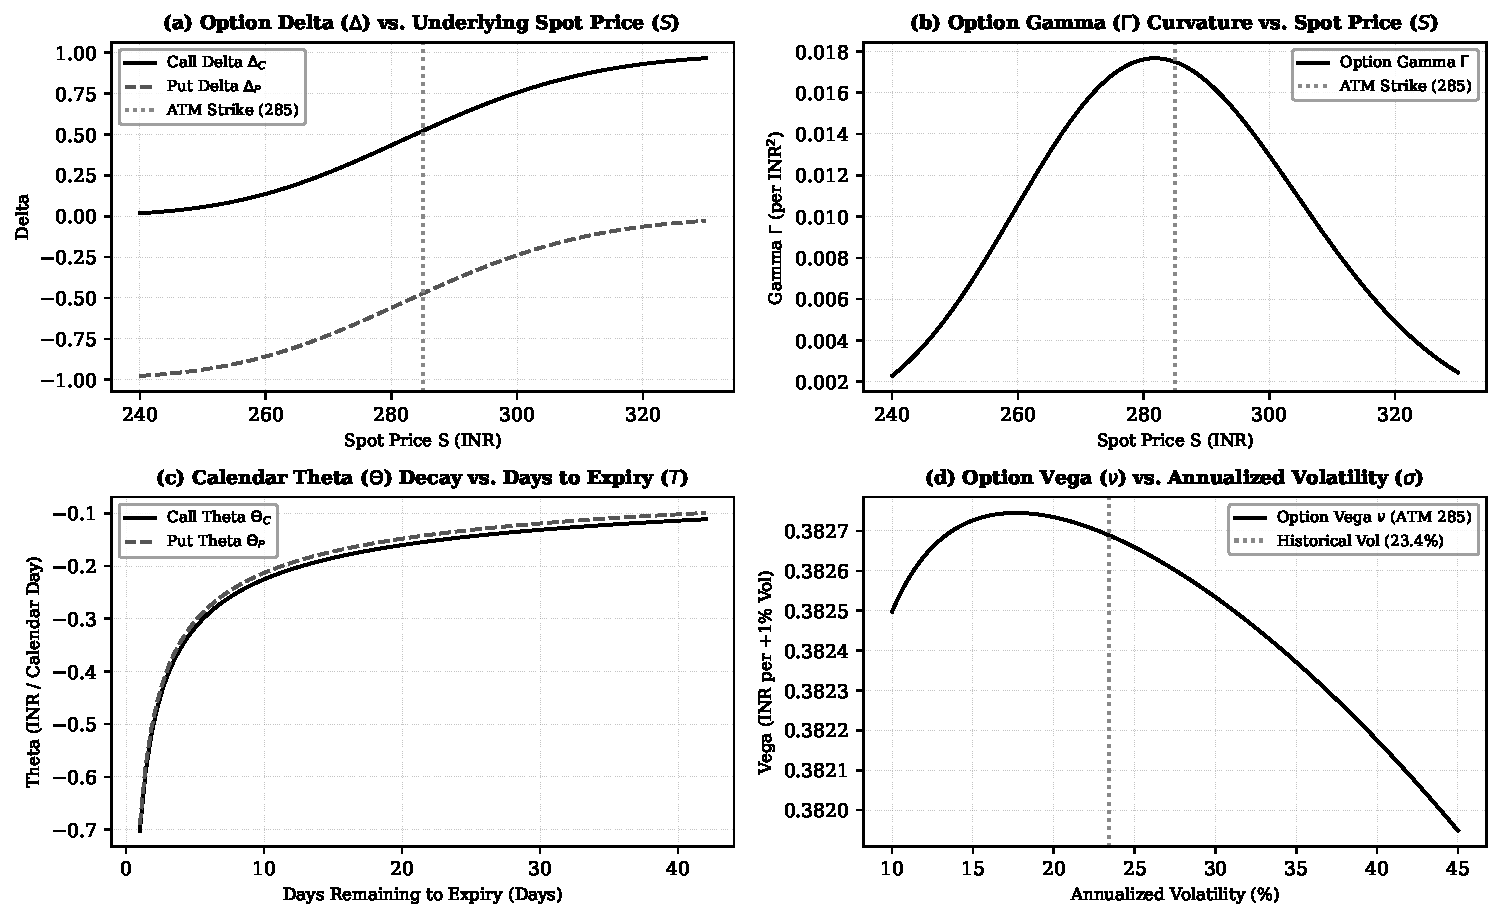
\includegraphics[width=\textwidth, height=7.2cm, keepaspectratio]{figures/fig1_fed_greeks_surface.pdf}
    \caption{4-Panel Sensitivity Profile of Option Greeks for ITC Limited. (A) Delta profile across spot prices; (B) Gamma curvature peaking sharply at-the-money ($S_0 = \text{\inr}285$); (C) Theta time decay per calendar day; (D) Vega sensitivity across spot prices peaking at-the-money.}
    \label{fig:fed_greeks_surface}
\end{figure}
\vspace{-0.5em}

\subsection{Risk Sensitivity Analysis}

As demonstrated in Figure~\ref{fig:fed_greeks_surface}, Gamma reaches its absolute maximum of $\Gamma = 0.0182$ at the ATM strike of \inr 285.00. For an equity option market maker, high Gamma implies severe non-linear delta slippage during market dislocations, requiring frequent rehedging. Daily Theta decay peaks at $-\text{\inr}0.114$ per share for ATM contracts (\inr 196.65 per lot per day), creating significant time-decay drag for long option holders.

\clearpage
